%-----------------------------------------------------------------------------%
\chapter{\babDua}
%-----------------------------------------------------------------------------%

%-----------------------------------------------------------------------------%
\section{Ekspresi Gen}
%-----------------------------------------------------------------------------%
Percobaan microarray, mengukur tingkat aktivitas gen di dalam sebuah jaringan sel. Sehingga dapat memberikan informasi berdasarkan aktivitas di dalam jaringan yang bersangkutan. Data ini didapatkan dengan cara mengukur banyaknya mRNA yang diproduksi pada saat proses transkripsi DNA, dimana dapat diukur seberapa aktif atau seberapa berfungsinya gen tersebut dalam sebuah jaringan \citep{elloumi2011algorithms}. Karena kanker berhubungan dengan berbagai macam aktivitas penyimpangan regulasi pada sel, maka data ekspresi gen pada kanker merefleksikan penyimpangan regulasi tersebut. Untuk menangkap keabnormalan ini, percbaan microarray, dimana dapat mengukur secara simultan dari level ekspresi ratusan bahkan ribuan ekspresi gen dapat digunakan untuk mengidentifikasi kanker. Percobaan microarray sering dipakai untuk membandingkan profil ekspresi gen pada sel yang terkena kanker, dibandingkan dengan sel yang normal pada berbagai macam percobaan. Percobaan microarray digunakan untuk mengidentifikasi ekspresi yang berbeda pada dua percobaan, yang biasanya berupa data tes dan data kontrol.\\
\begin{figure}
	\centering
	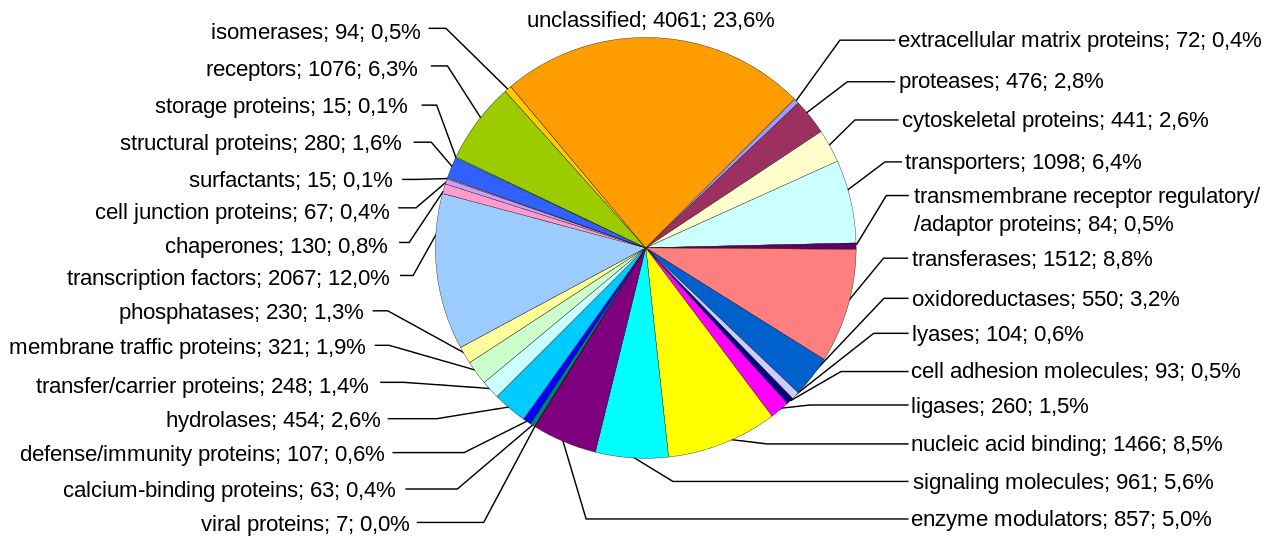
\includegraphics[width=0.50\textwidth]
		{pics/gbr2_1.png}
	\caption{Ada 23,6\% dari keseluruhan fungsi gen yang belum diketahui, sehingga pengetahuan tentang fungsi gen masih belum lengkap. \citep{haggstrom2014diagram}}
	\label{fig:gbr2.1}
\end{figure}

Data ekspresi gen yang masih mentah didapatkan dari percobaan di laboratorium menggunakan alat yang dinamakan dengan alat Genchip microarray. Data tersebut kemudian dilakukan pemrosesan awal untuk mendapatkan sebuah matriks ekspresi gen. Matriks ini memiliki data kolom dan baris, dimana kolom berisi data eksperimen, dan baris berisi nilai ekspresi pada tiap-tiap gen (gambar 2.2) [Babu, 2004].

\begin{figure}
	\centering
	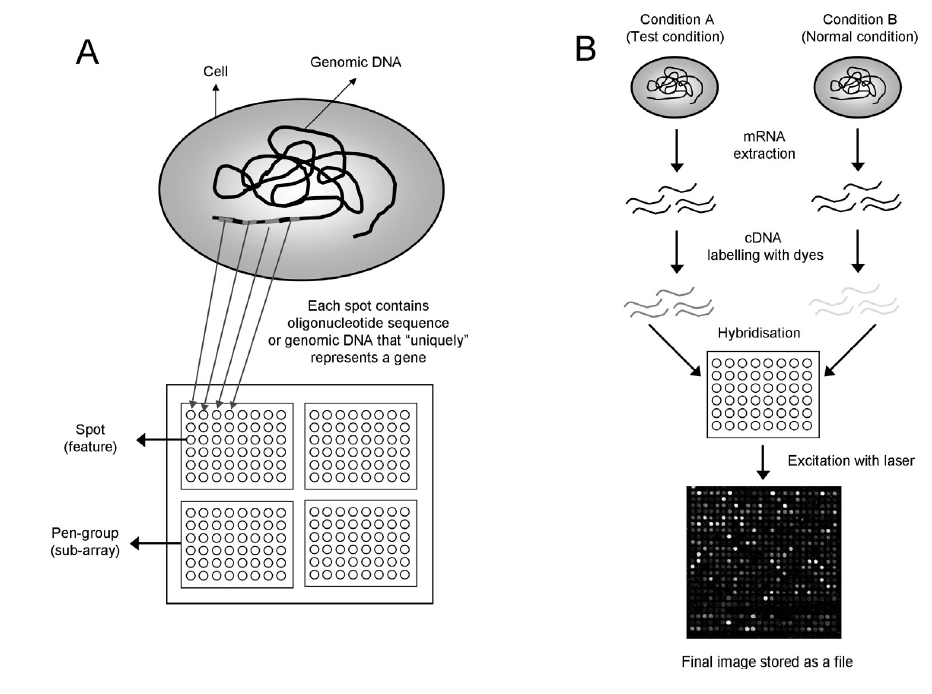
\includegraphics[width=0.50\textwidth]
		{pics/gbr2_2.png}
	\caption{Proses Keseluruhan Percobaan Microarray.\citep{babu2004introduction}}
	\label{fig:gbr2.2}
\end{figure}

\todo{tambahkan dua gambar yang digambar sendiri}

Karena data microarray yang didapatkan dapat mencapai ribuan ekspresi dalam satu waktu secara simultan, maka data ini dapat sangat membantu dalam mengidentifikasi penyakit. Akan tetapi, hasil yang didapat dengan menganalisa beberapa data microarray yang dilakukan oleh dua percobaan yang berbeda tetapi dengan tujuan yang sama, dapat menghasilkan hasil yang sangat berbeda. Salah satu alasannya adalah terbatasnya sampel dan terlalu banyaknya profil ekspresi gen. Sehingga diperlukan metode testing statistik untuk memastikan bahwa data microarray tersebut memiliki tingkat signifikansi yang cukup, dan dipastikan bahwa perbedaan tersebut memang karena eksperimen, bukan karena kerusakan alat atau kesalahan prosedur eksperimen.

%-----------------------------------------------------------------------------%
\section{Pemrosesan Data Microarray}
%-----------------------------------------------------------------------------%
Data yang dihasilkan dari alat microarray ini berupa citra yang perlu diproses lebih lanjut. Sebelum data ekspresi gen dapat dianalisa lebih lanjut, perlu dilakukan pemrosesan awal yang berupa (i) perbaikan background, (ii) normalisasi data dan kemudian (iii) penyaringan data.
\begin{enumerate}
\item{\textbf{Perbaikan Background}}\\
Perbiakan background ini ditujukan untuk menghilangkan titik-titik noise yang tidak berasal dari proses hibridisasi. Metode untuk perbaikan background ini banyak diajukan dalam penelitian. [15]
\item{\textbf{Normalisasi}}\\
Tujuan dari normalisasi adalah untuk mengatur bias yang dihasilkan oleh variasi proses percobaan microarray. Metode normalisasi data microarray ada banyak, dan pada penelitian ini akan digunakan normalisasi standar untuk data microarray.
\item{\textbf{Penyaringan data}}
Tidak semua data yang didapat dari percobaan microarray bagus, kadangkala terjadi kesalahan alat dan noise yang diakibatkan oleh alat, oleh karena itu perlu disaring, mana data yang disebabkan oleh proses biologi, dan mana yang disebabkan oleh noise alat.
\item{\textbf{Missing Value Imputation}}\\
Tidak semua data ekspresi gen dapat kita dapatkan, dikarenakan rumitnya percobaan microarray, kadangkala data tidak kita dapatkan, oleh sebab itu diperlukan metode untuk melakukan pendekatan statistic dalam memberikan perkiraan isi data dalam titik data yang hilang tersebut.
\item{\textbf{Seleksi Fitur}}\\
Setelah proses diatas, diperlukan teknik untuk menseleksi fitur pada data microarray. Ada banyak metode yang sudah diusulkan oleh para peneliti. Seperti pada table 1 dibawah. Dan pada titik inilah penelitian ini dijalankan. Diharapkan penelitian ini menghasilkan metode reduksi dimensi untuk data microarray.

\end{enumerate}

%-----------------------------------------------------------------------------%
\section{Ekstraksi Fitur dan Seleksi Fitur Pada Penelitian Sebelumnya}
%-----------------------------------------------------------------------------%
\todo{tulis tabel perbandingan seleksi fitur}


%-----------------------------------------------------------------------------%
\section{Deep Learning}
%-----------------------------------------------------------------------------%
\todo {tuliskan secara singkat tentang deep learning}

%-----------------------------------------------------------------------------%
\section{Restricted Boltzmann Machine}
%-----------------------------------------------------------------------------%
\todo{tuliskan secara detail tentang rbm}

%-----------------------------------------------------------------------------%
\section{Deep Believe Network}
%-----------------------------------------------------------------------------%
\todo{tuliskan secara detail tentang dbn}

%-----------------------------------------------------------------------------%
\section{Maximum Likelihood Estimation}
%-----------------------------------------------------------------------------%
\todo{tuliskan secara detail tentang MLE}
$    \mathcal{L}(\theta\,|\,x_1,\ldots,x_n) = f(x_1,x_2,\ldots,x_n|\theta) = \prod\limits_{i=1}^n f(x_i|\theta)  $

Thus, the extrema of $\mathcal{L}$  are equivalent to the extrema of $ \log \mathcal{L} $ :

   \begin{equation}
   \log \mathcal{L}(\theta\,|\,x_1,\ldots,x_n) = \sum\limits_{i=1}^n \log f(x_i|\theta) 
   \end{equation}

From which the maximum likelihood estimator $\hat{\theta}_{\textnormal{MLE}}$  is defined as:

   \begin{equation}
   \hat{\theta}_{\textnormal{MLE}} = \underset{\theta}{\arg\max} \sum\limits_{i=1}^n \log f(x_i|\theta) 
   \end{equation}

As an aside, Bayesians will remind us we can generalized into a MAP estimator, given uniform prior $ g(\theta) $ :

  \begin{equation}
   \underset{\theta}{\arg\max} \sum\limits_{i=1}^n \log f(x_i|\theta)  = \underset{\theta}{\arg\max} \log(f|\theta) = \underset{\theta}{\arg\max} \log(f|\theta) g(\theta) = \hat{\theta}_{\textnormal{MAP}} 
  \end{equation}

From which optimization and real analysis reminds us of the following equivalence, for all x:

   \begin{equation}
   \underset{x}{\arg\max} (x)  = \underset{x}{\arg\min} (-x) 
   \end{equation}

Thus, the following are equivalent:

   \begin{equation}
   \underset{\theta}{\arg\max} \sum\limits_{i=1}^n \log f(x_i|\theta) = \underset{\theta}{\arg\min} - \sum\limits_{i=1}^n \log f(x_i|\theta) = \hat{\theta}_{\textnormal{MLE}} 
   \end{equation}

%-----------------------------------------------------------------------------%
\section{Multi Layer Perceptron}
%-----------------------------------------------------------------------------%
\todo{tuliskan secara detail tentang dbn}

%-----------------------------------------------------------------------------%
\section{Logistic Regression}
%-----------------------------------------------------------------------------%
\todo{tuliskan secara detail tentang dbn}
